\documentclass[problems]{esg8012pset} 
  \usepackage{amsmath}
  \usepackage{amssymb}
  \usepackage{enumerate}
  \usepackage{graphicx}
  \usepackage{hyperref}
  %\usepackage{siunitx}
  \providecommand{\uvec}[1]{{\hat{\bf{#1}}}}
  \usepackage{pgf,tikz}
  \usetikzlibrary{arrows}
  \makeatletter
  \newcommand{\interitemtext}[1]{%
    \begin{list}{}
     {\itemindent=0mm\labelsep=0mm
     \labelwidth=0mm\leftmargin=0mm
     \addtolength{\leftmargin}{-\@totalleftmargin}}
      \item #1
    \end{list}
  }
  \makeatother
  \renewcommand{\d}{\,d}
  \providecommand{\norm}[1]{\lVert#1\rVert}
\classname{Physics 8.012} 
\semester{Fall 2010} 
\problemsetnumber{8} 
\date{Month Day\csname latex@error\endcsname {Date not yet decided}} 
\duedate{Friday, Month Day \csname latex@error\endcsname {Date not yet decided}} 
\readingassignment{Kleppner and Kolenkow, \emph {An Introduction to Mechanics}, Chapter Six} 
\begin{document}
\section*{Problem 1: K\&K 6.1}
  \begin{enumerate}[(a)]
    \item Show that if the total linear momentum of a system of particles is zero, the angular momentum of the system is the same about all origins. Explain how you may apply this result involving an elastic collision of two rigid bodies.
    \item Show that if the total force on a system of particles is zero, the torque on the system is the same about all origins. Explain how you can use this result for static equilibrium problems.
  \end{enumerate}
\section*{Problem 2: K\&K 6.2}
  A drum of mass $m_A$ and radius $a$ rotates freely with initial angular velocity $\omega_{A,0}$. A second drum with mass $m_B$ and radius $b > a$ is mounted on the same axle and is at rest, although it is free to rotate. A thin layer of sand with mass $m_S$ is distributed on the inner surface of the smaller drum. At $t = 0$, small perforations in the inner drum are opened. The sand starts to fly out at a constant rate $\lambda$ and sticks to the outer drum. Find the subsequent angular velocities of the two drums $\omega_A$ and $\omega_B$. Ignore the transit time of the sand.
  \begin{center}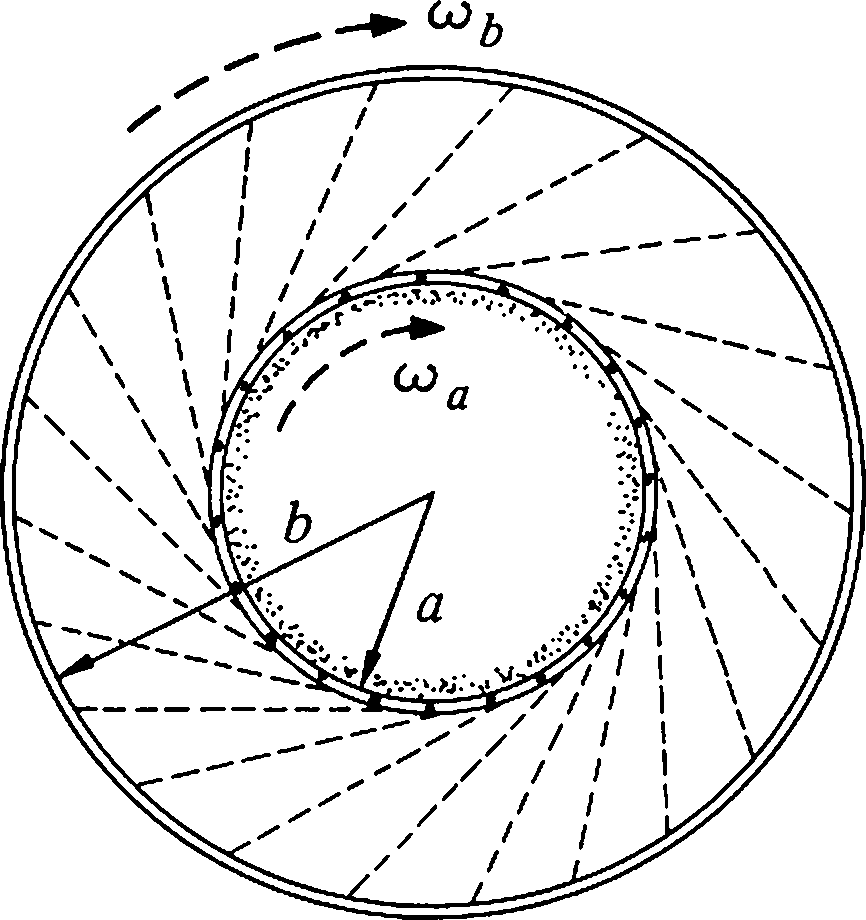
\includegraphics[width=0.2\textwidth]{ps08_1}\end{center}
\section*{Problem 3: K\&K 6.4}
  A spaceship is sent to investigate a planet of mass $m_p$ and radius $r_p$. While hanging motionless in space at a distance $5 r_p$ from the center of the planet, the ship fires an instrument package with speed $v_0$. The package has mass $m_i$ which is much smaller than the mass of the spacecraft. The package is launched at an angle $\theta$ with respect to a radial line between the center of the planet and the spacecraft. For what angle $\theta$ will the package just graze the surface of the planet.
  \begin{center}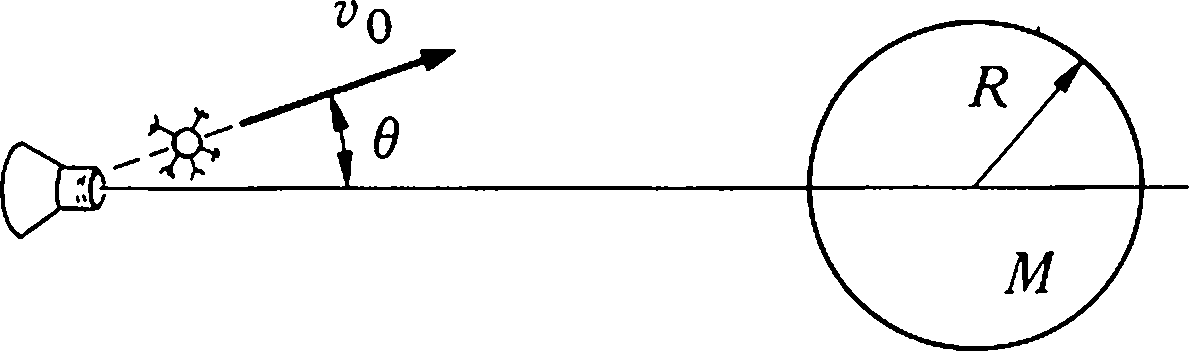
\includegraphics[width=0.4\textwidth]{ps08_2}\end{center}
\section*{Problem 4: K\&K 6.6}
  A person of mass $m$ is standing on a railroad car which is rounding an unbanked turn of radius $R$ at a speed $v$. His center of mass is at a height of $L$ above the car midway between his feet which are separated by a distance of $d$. The man is facing the direction of motion. What is the magnitude of the normal forces on each foot?
  \begin{center}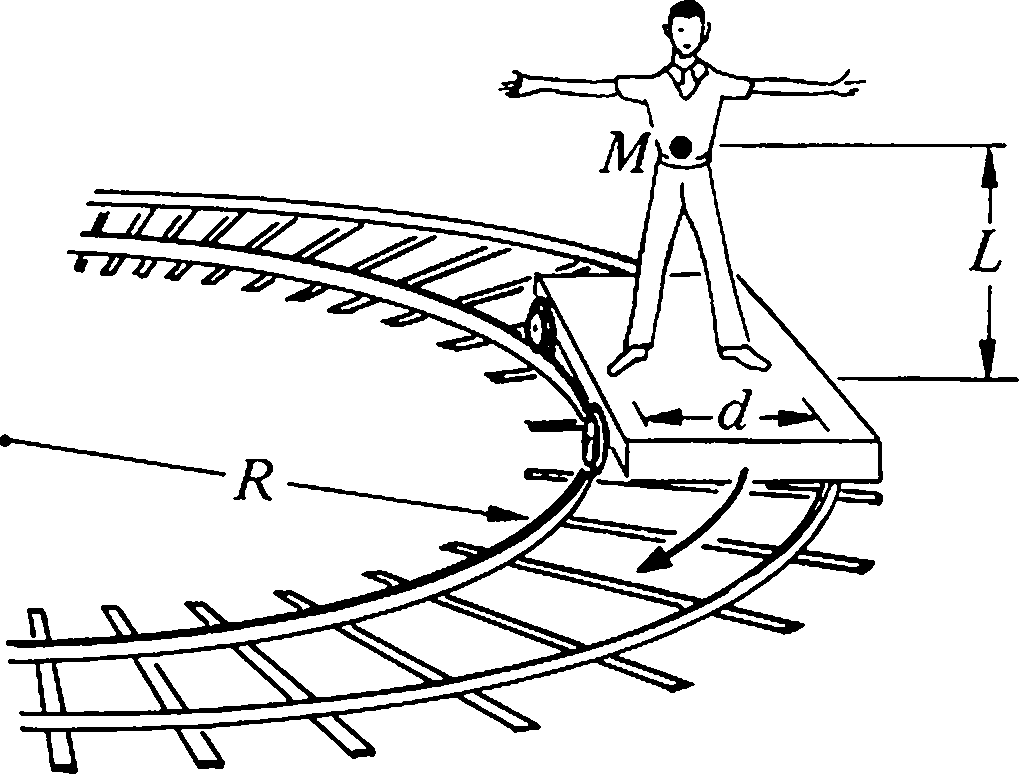
\includegraphics[width=0.4\textwidth]{ps08_3}\end{center}
\section*{Problem 5: K\&K 6.7}
  \begin{enumerate}[(a)]
    \item Find the moment of inertia of a thin sheet of metal of mass $m$ in the shape of an isosceles right triangle about an axis that passes through one vertex of the sheet, perpendicular to the plane of the sheet. The length of the two equal sides is $s$.
    \item Find the moment of inertia of a thin sheet of metal of mass $m$ in the shape of an isosceles right triangle about an axis that passes through the same vertex of the sheet, but aligned along one side of length $s$ (in the plane of the sheet).
  \end{enumerate}
\section*{Problem 6: K\&K 6.10}
  A cylinder of mass $m$ and radius $R$ is rotated in a V groove with constant angular velocity $\omega_{0}$.
The coefficient of friction between the cylinder and the surface is $\mu$. What external torque must be applied to the cylinder to keep it rolling?
  \begin{center}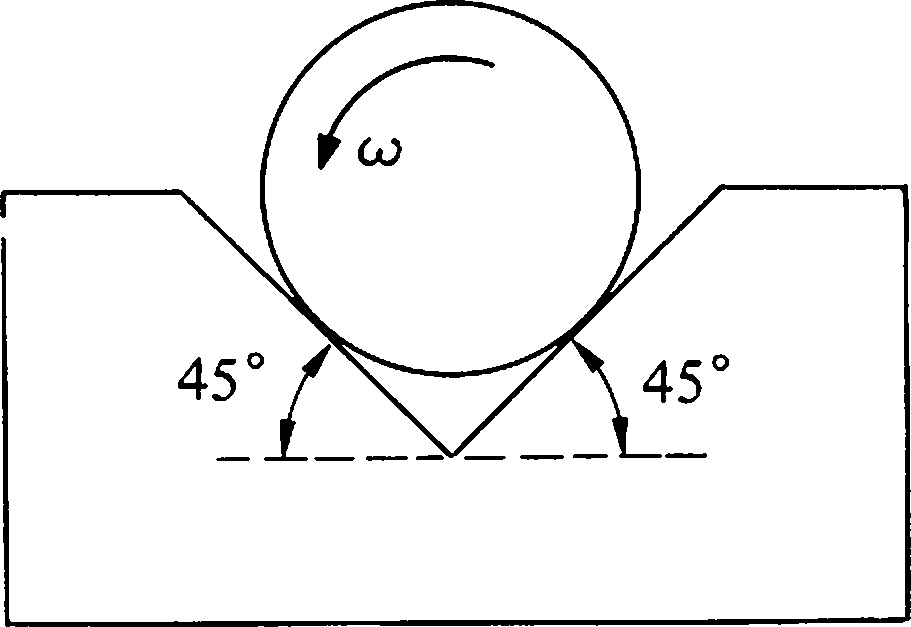
\includegraphics[width=0.3\textwidth]{ps08_4}\end{center}
\section*{Problem 7: K\&K 6.13}
  A body of particle of mass $m$ (treat it as a point like particle) is attached to a post of radius $R$ by a string. Initially it is a distance $r_0$ from the center of the post and it is moving tangentially with a speed $v_0$. In case (a) the string passes through a hole in the center of the post at the top. The string is gradually shortened by drawing it through the hole. In case (b) the string wraps around the outside of the post. What quantities remain constant in each case? Find the final speed of the body when it hits the post for each case.
  \begin{center}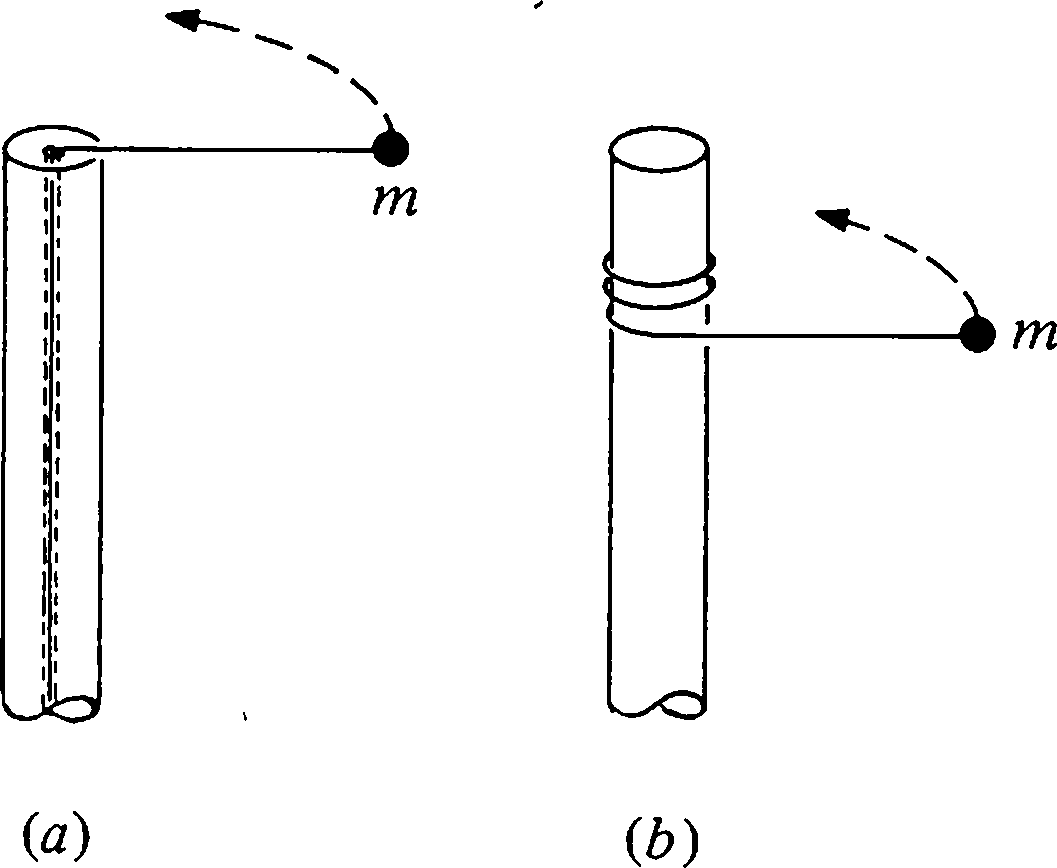
\includegraphics[width=0.3\textwidth]{ps08_5}\end{center}
\end{document}
